\chapter{Analiza wymagań}

\section{Wstęp}

%TODO Alternatywna wersja 

Wraz z rozwojem handlu konieczne stało się stworzenie miejsca w którym towary
będą składowane przed zakupem przez klienta. W przypadku małych magazynów to
pracownicy są w stanie nim efektywnie zarządzać i efektywnie wyszukiwać 
znajdujące się w nim towary. Jednak co dzieje się w przypadku, gdy liczba towarów
przechowywanych w magazynie jest bardzo duża? Konieczne staje się stworzenie
systemu który umożliwi pracownikom prostsze i bardziej efektywne zarządzanie
towarami znajdującymi się w magazynie.

Głównym zadaniem systemu do zarządzania magazynem jest przechowywanie ilości
poszczególnych towarów, odznaczanie dostaw jak i również sprzedaży
towarów klientom. Powinien również przechowywać niezbędne informacje o
dostawcach, towarach oraz klientach.

\subsection{Przeznaczenie systemu}

Głównym zadaniem systemu jest ułatwienie zarządzania magazynem pracownikom
magazynu, poprzez umożliwienie zarządzania klientami, dostawcami, towarami a
także zamówieniami sprzedaży jak i zakupu. System ten nie jest specjalizowany
pod konkretną dziedzinę handlu -- ma on umożliwiać przechowywanie i
zarządzanie informacjami o towarach dowolnego typu. 

%%%%%%%%%% DZIEDZINA PROBLEMU
\section{Dziedzina problemu}
Poniżej przedstawione zostały kluczowe pojęcia i procesy charakteryzujące system obsługi magazynu.

\subsection{Towary}
Towar jest podstawową jednostką przechowywaną w magazynie. Każdy towar jest opisany przez następujące cechy:
\begin{itemize}
	\item nazwa,
	\item kod kreskowy,
	\item kategoria,
	\item jednostka miary,
	\item stan początkowy (początkowa ilość towaru w magazynie),
	\item cena sprzedaży.
\end{itemize}

Możliwe są następujące operacje:
\begin{itemize}
	\item dodawanie towaru,
	\item edytowanie towaru z wyłączeniem bezpośredniej edycji stanu początkowego, który jest cechą ustalaną na podstawie dokumentów PZ, WZ oraz korekt magazynu,
	\item usuwanie towarów, które nie znajdują się w żadnym z dokumentów PZ, WZ lub korekcie magazynu.
\end{itemize}

Ponadto dla każdego towaru możliwe jest określenie stanu minimalnego oraz maksymalnego w magazynie, od którego zależna będzie możliwość dokonania operacji przyjęcia zamówienia, wydania zamówienia oraz korekty stanu magazynu.

\subsection{Dokumenty}
W systemie wyróżnione są trzy typy dokumentów: PZ, WZ oraz korekta stanu magazynu.

\subsubsection{PZ}
Dokument PZ jest dokumentem powiązanym z procesem przyjęcia towaru.
Dokument PZ zawiera:
\begin{itemize}
	\item numer dokumentu: PZnr\_kolejny\_dokumentu/rok, np: PZ1/2003,
	\item dane wystawcy (magazynu),
	\item dane kontrahenta,
	\item datę operacji,
	\item dane towarów wraz z ilością przyjętych towarów -- wartość ta dodaje się do stanu towaru w magazynie,
	\item cenę towaru, ustalaną indywidualnie dla każdego dokumentu PZ,
	\item łączną cenę towarów.
\end{itemize}

\subsubsection{WZ}
Dokument WZ jest dokumentem powiązanym z procesem wydania towaru.
Dokument WZ zawiera:
\begin{itemize}
	\item numer dokumentu: WZnr\_kolejny\_dokumentu/rok, np: WZ1/2003,
	\item dane wystawcy (magazynu),
	\item dane kontrahenta,
	\item datę operacji,
	\item dane towarów wraz z ilością przyjętych towarów -- wartość ta odejmuje się do stanu towaru w magazynie,
	\item cenę towaru, ustalaną indywidualnie dla każdego dokumentu WZ (cena towaru z danych towaru to tylko sugestia),
	\item łączną cenę towarów.
\end{itemize}

\subsubsection{Korekta stanu magazynu}
\begin{itemize}
	\item data korekty,
	\item numer dokumentu: Knr\_kolejny\_dokumentu/rok, np. K1/2013,
	\item dane towarów, których stan podlega korekcie,
	\item nowy stan towaru,
	\item suma modyfikowanej ilości towarów na dokumencie.
\end{itemize}

\subsubsection{Korekta PZ}
Korekta PZ jest dokumentem analogicznym do dokumentu PZ, z zastrzeżeniem, iż odnosi się ona do już istniejącego dokumentu PZ oraz dane z korekty PZ muszą być zgodne z danymi dokumentu PZ do którego ta korekta się odnosi -- w korekcie może znaleźć się tylko podzbiór towarów z dokumentu PZ a ilości poszczególnych towarów na korekcie nie mogą przekraczać ilości towarów oryginalnego dokumentu.

Ponadto:
\begin{itemize}
	\item numer dokumentu: PZknr\_kolejny\_dokumentu/rok, np PZk1/2013 (numer kolejny dokumentu nie jest w żaden sposób powiązany z jakimkolwiek numerem istniejącego dokumentu),
	\item cena towaru w korekcie PZ ustalana jest niezależnie od ceny z oryginalnego dokumentu PZ,
	\item ilość towaru w korekcie PZ odejmuje się od stanu towaru w magazynie.
\end{itemize}

\subsubsection{Korekta WZ}
Korekta WZ jest dokumentem analogicznym do dokumentu WZ, z zastrzeżeniem, iż odnosi się ona do już istniejącego dokumentu WZ oraz dane z korekty WZ muszą być zgodne z danymi dokumentu WZ do którego ta korekta się odnosi -- w korekcie może znaleźć się tylko podzbiór towarów z dokumentu WZ a ilości poszczególnych towarów na korekcie nie mogą przekraczać ilości towarów oryginalnego dokumentu.

Ponadto:
\begin{itemize}
	\item numer dokumentu: WZknr\_kolejny\_dokumentu/rok, np WZk1/2013 (numer kolejny dokumentu nie jest w żaden sposób powiązany z jakimkolwiek numerem istniejącego dokumentu),
	\item cena towaru w korekcie WZ ustalana jest niezależnie od ceny z oryginalnego dokumentu WZ,
	\item ilość towaru w korekcie WZ dodaje się od stanu towaru w magazynie.
\end{itemize}

\subsection{Przyjęcie towaru}
Z procesem przyjęcia towaru powiązane są następujące operacje:
\begin{itemize}
	\item utworzenie dokumentu PZ,
	\item edycja dokumentu PZ -- dowolne pole, zmiany ilości przyjętego towaru wpływają na stan towaru w magazynie,
	\item usunięcie dokumentu PZ -- usunięcie dokumentu PZ powoduje aktualizację (odjęcie) ilości towarów, które były uwzględnione w tym dokumencie.
\end{itemize}

\subsection{Wydanie towaru}
Z procesem wydania towaru powiązane są następujące operacje:
\begin{itemize}
	\item utworzenie dokumentu WZ,
	\item edycja dokumentu WZ -- dowolne pole, zmiany ilości przyjętego towaru wpływają na stan towaru w magazynie,
	\item usunięcie dokumentu WZ -- usunięcie dokumentu WZ powoduje aktualizację (dodanie) ilości towarów, które były uwzględnione w tym dokumencie.
\end{itemize}

Dodatkowo można wskazać przyjęcie towaru, do którego odnosi się to wydanie towaru: wtedy możliwe jest wskazanie wydawanego towaru, który był kiedyś przyjęty za pewną kwotę, a tym samym możliwe jest obliczenie zysku ze wydania towaru/wskazanie marży z towaru)

\section{Aktorzy}

Aktorzy w zaprojektowanym systemie zostali podzieleni na dwie grupy: aktorów
osobowych oraz aktorów nieosobowych. Do aktorów osobowym można zaliczyć
wszystkich użytkowników projektowanego systemu, aktorami nieosobowymi są
natomiast wszystkie systemy zewnętrzne współpracujące z projektowanym systemem.
Poniższy diagram przedstawia hierarchię aktorów osobowych w systemie:

\begin{figure}[h]
    \begin{center}
    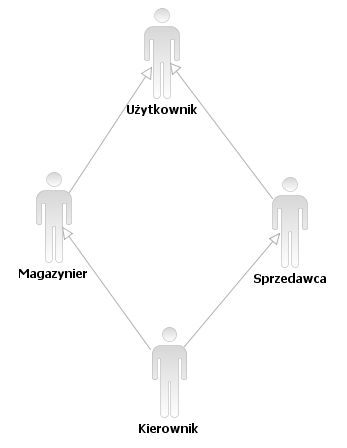
\includegraphics[scale=0.75]{../img/diagramDziedziczenia.png}
    \end{center}
    \label{fig:diagramDziedziczenia}
    \caption{Diagram przedstawiający aktorów w systemie}
\end{figure}
\FloatBarrier

\section{Wymagania funkcjonalne}

Niniejsze rozdział zawiera wymagania funkcjonalne jakie powinien spełniać
projektowany system. Wymagania te zostały podzielone na odpowiednie grupy wymagań.
Grupy wymagań zawierają bardziej szczegółowe wymagania, takie jak edycja czy
usuwanie danych. W tabeli umieszczone zostały również informacje o priorytecie
wymagania oraz ryzyku realizacji i aktorach.

%\arrayrulecolor{line}
%\rowcolors{2}{cell}{white}

\begin{table}[ht]
	 \begin{center}
% 	    \rowcolors{1}{}{light-blue}
	    \begin{tabular}{| l | l | l | l | l |}%\toprule
	    	\hline
		    \textbf{LP.} & \textbf{Nazwa}  & \textbf{Priorytet} & \textbf{Ryzyko} &
		    \textbf{Aktor} \\
		    \hline
			1 & Zarządzanie pracownikami & wysoki & niskie & kierownik \\
		    1.1 & Dodawanie pracownika & wysoki & niskie & kierownik \\
		    1.2 & Edycja danych pracownika & wysoki & niskie & kierownik \\ 	
		    1.3 & Usuwanie danych pracownika & wysoki &niskie & kierownik \\
		    \hline
		    2 & Zarządzanie danymi towarów & wysoki & niskie & magazynier \\
		    2.1 & Dodawanie towaru & wysoki &  niskie & magazynier \\
		    2.2 & Edycja opisu towaru & wysoki & niskie & magazynier \\
		    2.3 & Usuwanie danych towaru & wysoki & niskie & magazynier \\
            2.4 & Korekta stanu towaru & wysoki & niskie & magazynier \\
		    \hline
		   	3 & Zarządzanie danymi kontrahentów & wysoki & niskie & użytkownik \\
		   	3.1 & Dodawanie kontrahenta & wysoki & niski & użytkownik \\
		   	3.2 & Edycja danych kontrahenta & wysoki & niskie & użytkownik \\
		   	3.3 & Usuwanie danych kontrahenta & średni & niskie & użytkownik \\
		   	\hline
            4 & Przyjęcie na magazyn & wysoki & niskie & magazynier \\
		   	4.1 & Tworzenie dokumentu przejęcia towaru & wysoki & niskie & magazynier \\
		   	4.2 & Edycja dokumentu przyjęcia towaru & wysoki & niskie & magazynier \\
		   	4.3 & Usuwanie dokumentu przyjęcia towaru & wysoki & niskie & magazynier \\
		   	4.4 & Realizacja przyjęcia towaru & wysoki & niskie & magazynier \\
		   	4.5 & Korekta przyjęcia towaru & średni & niskie & magazynier \\
            \hline
		   	5 & Wydanie z magazynu & wysoki & niskie & sprzedawca \\
		   	5.1 & Tworzenie dokumentu wydania towaru & wysoki & niskie & sprzedawca \\
		   	5.2 & Edycja dokumentu wydania towaru & średni & niskie & sprzedawca \\
		   	5.3 & Usuwanie dokumentu wydania towaru & wysoki & niskie & sprzedawca \\
		   	5.4 & Realizacja wydania towaru & wysoki & niskie & sprzedawca \\
		   	5.5 & Korekta wydania towaru & średni & niskie & sprzedawca \\
		   	\hline
		   	6 & Zarządzanie raportami & średni & niskie & kierownik \\
		   	6.1 & Generowanie raportów o wydanych towarach & średni & niskie & kierownik \\
		   	6.2 & Generowanie raportów o przyjętych towarach & średni & niskie & kierownik \\
		   	\hline
	    \end{tabular}
	\end{center}
\end{table}
\FloatBarrier
\newpage
\section{Wymagania niefunkcjonalne}

Rozdział ten zawiera wymagania niefunkcjonalne dotyczące projektowanego systemu.
Wymagania zostały podzielone na kilka grup, przy każdym z wymagań został
określony priorytet oraz ryzyko.

\begin{table}[h]
	\begin{center}
		\begin{tabular}{| l | l | l | l |}
			\hline
			\textbf{Lp.} & \textbf{Nazwa} & \textbf{Priorytet} & \textbf{Ryzyko} \\
			\hline
			1 & Bezpieczeństwo & wysoki & niskie \\
			1.1 & Mechanizm uwierzytelniania użytkowników za pomocą & wysoki & niskie \\
			& loginu i hasła & & \\
			1.2 & Zróżnicowanie uprawnień do korzystania z systemu & wysoki & niskie \\
			1.3 & Zapisywanie historii przeprowadzanych transakcji & wysoki & niskie \\
			1.4 & Szyfrowanie haseł w bazie danych funkcją skrótu & wysoki & niskie \\
			\hline
			2 & Dostępność & wysoki & niskie \\
			2.1 & Dostępność systemu co najmniej 98\% w skali dnia & wysoki & niskie \\ 
			2.2 & Dostępność przez przeglądarkę & wysoki & niskie \\
			\hline
			3 & Elastyczność & wysoki & niskie \\
			3.1 & Architektura systemu umożliwia łatwą rozbudowę  & wysoki & niskie \\
			& i konserwacje & & \\
			3.2 & Możliwość integracji z innymi systemami używanymi & wysoki & niskie \\
			& w firmie & & \\
			
			\hline
			4 & Niezawodność & wysoki & niskie \\
			4.1 & Maksymalny czas powstania po awarii 2h & wysoki & niskie \\
			4.2 & Odtwarzanie uszkodzonych danych na podstawie & wysoki	& niskie \\
			& kopii zapasowych & & \\
			4.3 & Wykonywanie kopii zapasowych danych & wysoki & niskie \\
			\hline
			5 & Użyteczność & wysoki & niskie \\
			5.1 & Intuicyjny sposób obsługi systemy & wysoki & niskie \\
			5.2 & Przejrzysty system pomocy & wysoki & niskie \\
			\hline
			6 & Wydajność & wysoki & niskie \\
			6.1 & Przechowywanie informacji o transakcjach przez 3 lata & wysoki & niskie
			\\
			6.2 & Umożliwienie równoczesnej pracy przez 200 użytkowników & wysoki &
			niskie
			\\
			\hline
		\end{tabular}
	\end{center}
\end{table}
\FloatBarrier
